%!TEX root = ../../report.tex
\chapter{Appendix}
\label{appendix:learning_curves}
The estimated $\lambda$ values are shown in figure \ref{fig:all_learnings_sim_1} and \ref{fig:all_learnings_sim_2}. The estimated values in the plots are calculated by the average estimate in an area around the obstacles. The requirement for a cell to be used in the average was all parameters, the state and event scores, were above 0.5. As this method deviates from the scoring method used for comparison the result are not directly comparable.
The figures gives an overview of the speed of leaning but as many cells are included that might mainly learn based on noise is may not represent an accurate image of the learning accuracy.


\begin{figure}[htbp]
	\begin{subfigure}[t]{0.5\linewidth}
		\centering
		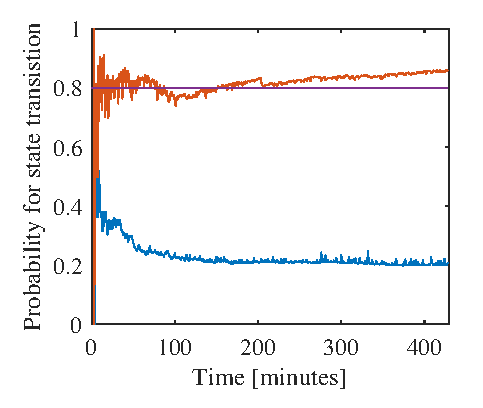
\includegraphics[width=1\linewidth]{chapters/appendix/figures/learning_curves/obs1}
		\caption{Obstacle number 1}
	\end{subfigure}
	\hspace*{\fill}
	\begin{subfigure}[t]{0.5\linewidth}
		\centering
		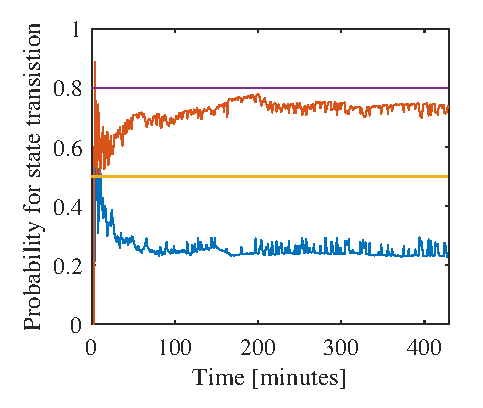
\includegraphics[width=1\linewidth]{chapters/appendix/figures/learning_curves/obs2}
		\caption{Obstacle number 2}
	\end{subfigure}


	\begin{subfigure}[t]{0.5\linewidth}
		\centering
		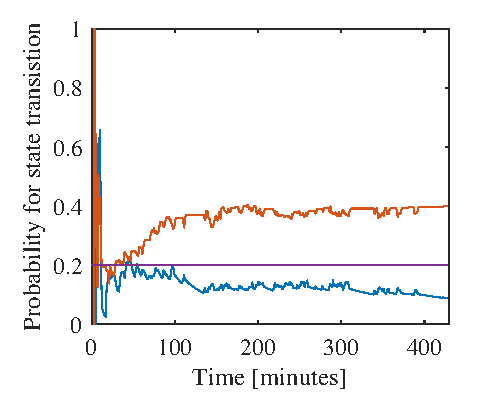
\includegraphics[width=1\linewidth]{chapters/appendix/figures/learning_curves/obs3}
		\caption{Obstacle number 3}
	\end{subfigure}
	\hspace*{\fill}
	\begin{subfigure}[t]{0.5\linewidth}
		\centering
		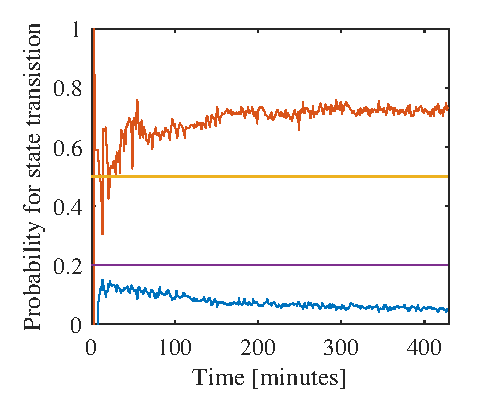
\includegraphics[width=1\linewidth]{chapters/appendix/figures/learning_curves/obs4}
		\caption{Obstacle number 4}
	\end{subfigure}
	
	\hspace*{\fill}
	\begin{subfigure}[t]{0.5\linewidth}
		\centering
		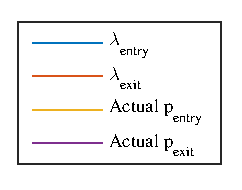
\includegraphics[scale = 1]{chapters/appendix/figures/learning_curves/legend}
		
	\end{subfigure}
	\hspace*{\fill}

	\caption{CAPTION}
	\label{fig:all_learnings_sim_1}
\end{figure}

\begin{figure}[htbp]
	\begin{subfigure}[t]{0.5\linewidth}
		\centering
		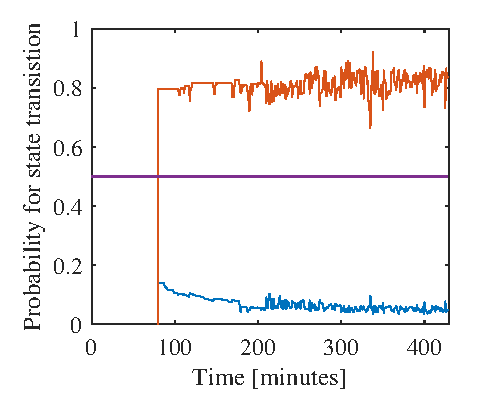
\includegraphics[width=1\linewidth]{chapters/appendix/figures/learning_curves/obs5}
		\caption{Obstacle number 5}
	\end{subfigure}
	\hspace*{\fill}
	\begin{subfigure}[t]{0.5\linewidth}
		\centering
		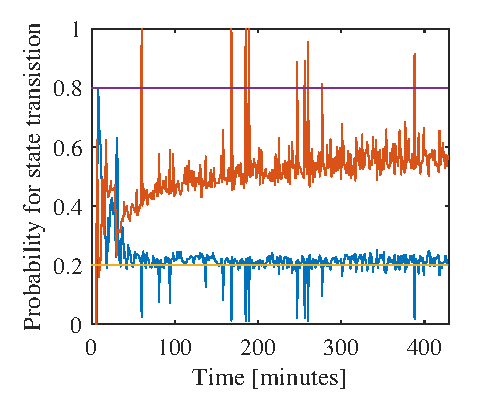
\includegraphics[width=1\linewidth]{chapters/appendix/figures/learning_curves/obs6}
		\caption{Obstacle number 6}
	\end{subfigure}
	
	\begin{subfigure}[t]{0.5\linewidth}
		\centering
		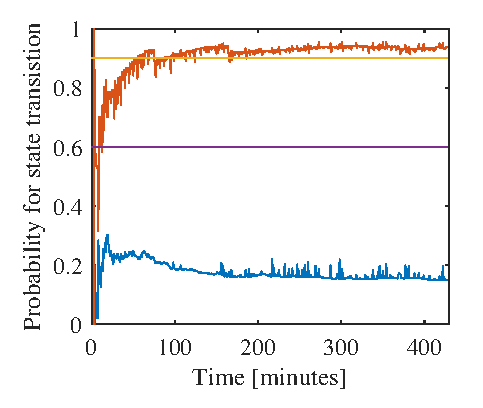
\includegraphics[width=1\linewidth]{chapters/appendix/figures/learning_curves/obs7}
		\caption{Obstacle number 7}
	\end{subfigure}
	\hspace*{\fill}
	\begin{subfigure}[t]{0.5\linewidth}
		\centering
		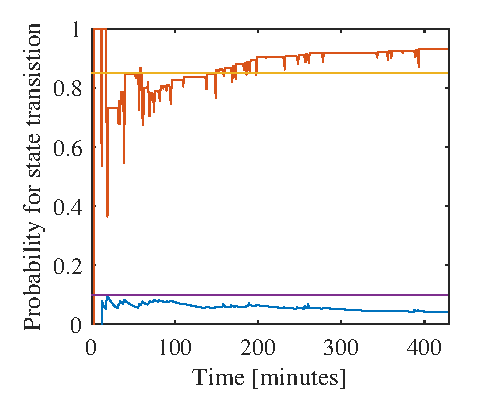
\includegraphics[width=1\linewidth]{chapters/appendix/figures/learning_curves/obs8}
		\caption{Obstacle number 8}
	\end{subfigure}


	\begin{subfigure}[t]{0.5\linewidth}
		\centering
		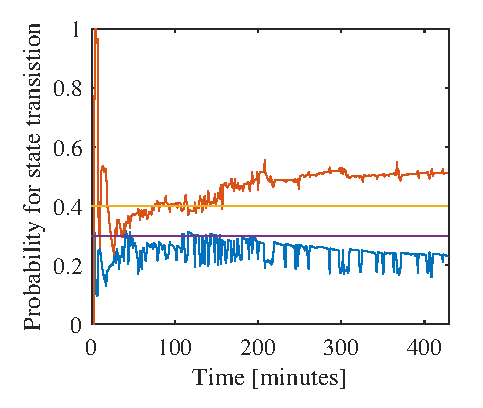
\includegraphics[width=1\linewidth]{chapters/appendix/figures/learning_curves/obs9}
		\caption{Obstacle number 9}
	\end{subfigure}
	\hspace*{\fill}
	\begin{subfigure}[t]{0.5\linewidth}
		\centering
		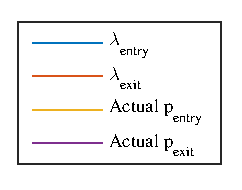
\includegraphics[scale = 1]{chapters/appendix/figures/learning_curves/legend}
	\end{subfigure}

	\caption{CAPTION}
	\label{fig:all_learnings_sim_2}
\end{figure}